\documentclass{report}
\usepackage[T1]{fontenc} % Fontes T1
\usepackage[utf8]{inputenc} % Input UTF8
\usepackage[backend=bibtex, style=ieee]{biblatex} % para usar bibliografia
\usepackage{csquotes}
\usepackage[portuguese]{babel} %Usar língua portuguesa
\usepackage{hyperref} % para autoref
\usepackage{graphicx}
\graphicspath{ {imagens/} }
\usepackage{mathptmx}
\usepackage{anyfontsize}
\usepackage{t1enc}
\usepackage[document]{ragged2e}
\usepackage[acronym]{glossaries}
\usepackage{glossaries}
\usepackage{enumitem}
\usepackage{array}
\usepackage{indentfirst}
\usepackage{listings}
\usepackage{color}
\usepackage[document]{xcolor}
\usepackage{tasks}

\setlength{\parindent}{4em}

\definecolor{dkgreen}{rgb}{0,0.6,0}
\definecolor{gray}{rgb}{0.5,0.5,0.5}
\definecolor{mauve}{rgb}{0.58,0,0.82}

\lstset{frame=tb,
  aboveskip=3mm,
  belowskip=3mm,
  showstringspaces=false,
  columns=flexible,
  basicstyle={\small\ttfamily},
  breaklines=true,
  breakatwhitespace=true,
  tabsize=3
}

\bibliography{bibliografia}

\makeglossaries

\newglossaryentry{packages}
{
    name=packages,
    description={Coleção de de programas ou subrotinas relativas a uma funcionalidade}
}

\newacronym{ua}{UA}{Universidade de Aveiro}
\newacronym{DETI}{DETI}{Departamento de Eletrónica, Telecomunicações, e Informática}
\newacronym{AETTUA}{AETTUA}{Associação de Eletrónica, Telecomunicações, e Telemática da Universidade de Aveiro}

\newacronym{RR}{RR}{Rodrigo Rosmaninho}
\newacronym{JS}{JS}{José Silva}

\begin{document}
%%
% Definições
%
\def\titulo{Funcionalidades do \LaTeX}
\def\data{13 de Novembro de 2017}
\def\autores{Rodrigo Rosmaninho, Jorge C. Silva}
\def\autorescontactos{(88802) r.rosmaninho@ua.pt, (88790) jorgemcsilva99@ua.pt}
\def\versao{1}
\def\departamento{Departamento de Eletrónica, Telecomunicações, e Informática}
\def\empresa{Universidade de Aveiro}
\def\logotipo{ua.pdf}
%
%%%%%% CAPA %%%%%%
%
\begin{titlepage}

\begin{center}
%
\vspace*{50mm}
%
{\Huge \titulo}\\ 
%
\vspace{10mm}
%
{\Large \empresa}\\
%
\vspace{10mm}
%
{\LARGE \autores}\\ 
%
\vspace{30mm}
%
\begin{figure}[h]
\center
\includegraphics{\logotipo}
\end{figure}
%
\vspace{30mm}
\end{center}
%
\begin{flushright}
\versao
\end{flushright}
\end{titlepage}

%%  Página de Título %%
\title{%
{\Huge\textbf{\titulo}}\\
{\Large \departamento\\ \empresa}
}
%
\author{%
    \autores \\
    \autorescontactos
}
%
\date{\data}
%
\maketitle

% \pagenumbering{roman}

%%%%%% RESUMO %%%%%%
\begin{abstract}
Neste documento sobre o sistema de preparação de texto denominado {\LaTeX}, iremos abordar, da forma mais breve e conscisa possível, uma variedade de funcionalidades do sistema, todas de grande utilidade, de forma a este documento servir de apoio a quem necessitar de uma introdução base a {\LaTeX}.
Essas funcionalidades podem ser divididas em três grandes grupos: \underline{formatação e estruturação do documento}, \underline{formatação de caractéres} e \underline{funcionalidades especiais}.\\

\vspace{2mm}
No primeiro grupo, serão tratadas formas de como é possível iniciar o documento e como definir a sua estrutura básica, dependendo da necessidade do redator. Aqui obterá informação sobre a capitulação, índices, bibliografia, etc...).Também será abordado a formatação textual, referente a paragrafização e outros aspetos de formatação textual.\\

\vspace{2mm}
No segundo grupo será tratado a formatação e transformação de caractéres. Aqui é possível encontrar informação sobre o tamanho dos caractéres, a sua font, etc...\\

\vspace{2mm}
No último grupo mencionado, é dada informação sobre algumas funcionalidades extra do {\LaTeX}. Isto engloba fórmulas matemáticas, criação de listas, tabelas e até inserção de imagens.\\

\vspace{2mm}
Apesar de ser um documento algo extenso, este apenas engloba uma fração de todas as funcionalidades do {\LaTeX}, mas o nosso objetivo é, desde já criar um documento de fácil leitura, e que seja capaz de fornecer ao leitor as bases necessárias para iniciar a própria redação de documentos em {\LaTeX}.
\end{abstract}

%%%%%% Agradecimentos %%%%%%
% Segundo glisc deveria aparecer após conclusão...
\renewcommand{\abstractname}{Agradecimentos}
\begin{abstract}
Gostaríamos de agradecer a: 

\begin{description}
	\item[\acrshort{AETTUA} e Professor Miguel Oliveira e Silva], pelo workshop de \LaTeX que ocorreu no dia 14 de Novembro, e que nos ajudou muito na realização deste trabalho.
	\item[Professor Auxiliar António Manuel Adrego da Rocha ], pela aula elucidante que nos foi dada sobre \LaTeX, sem a qual não conseguiríamos ter completado este relatório.
	\item[\acrshort{DETI}], pela cedência de salas livres nas quais pudemos elaborar o relatório em conjunto.
	\item[Professor Auxiliar João Paulo Barraca], pelo esclarecimento de variadas dúvidas sobre este trabalho de aprofundamento.
\end{description}
\end{abstract}


\tableofcontents
\listoftables
\listoffigures


%%%%%%%%%%%%%%%%%%%%%%%%%%%%%%%
\clearpage
\pagenumbering{arabic}

%%%%%%%%%%%%%%%%%%%%%%%%%%%%%%%%
\chapter{Introdução}
\label{chap.introducao}

O tema deste relatório é \textbf{Funcionalidades do \LaTeX} e, como já foi dito no resumo, o seu objetivo é ajudar a ensinar as bases desta linguagem, para que quem o leia possa depois redigir os seus próprios documentos em \LaTeX 

Este relatório está dividido em quatro capítulos para além desta Introdução.

\begin{description}
	\item[Capítulo \ref{chap.estrutrura}] - São apresentados diferentes formas de estruturar um documento em \LaTeX;
	\item[Capítulo \ref{chap.texto}] - São descritas variadas formas de manipulação de texto;
	\item[Capítulo \ref{chap.mat}] - Exemplificação de introdução de fórmulas matemáticas simples e complexas.
	\item[Capítulo \ref{chap.listas,tabelas e imagens}] - É ensinado o processo de introdução de Listas, Tabelas, e Imagens.
\end{description}

Finalmente, no \autoref{chap.conclusao} são apresentadas
as conclusões do trabalho.

\chapter{Estrutura de um Documento}
\label{chap.estrutrura}

Ao elaborar qualquer tipo de documento em \LaTeX é importante saber a estrutura a que o ficheiro \textbf{.tex} em causa deve obedecer. Ou seja, os comandos indispensáveis à realização de um relatório. 


Para além disso, existem comandos para alterar a estrutura e hierarquia do documento em si, como, por exemplo:

\begin{itemize}
	\item Páginas de Capa
	\item Índices
	\item Capítulos
	\item Secções, Sub-Secções
	\item Bibliografias
\end{itemize}
  

\section{Estrutura de um ficheiro \textbf{.tex}}

\subsection{documentclass}

Todos os documentos em \LaTeX têm que conter os comandos:  ~\cite{estrutura}

\begin{lstlisting}
\documentclass[options]{class}

\begin{document}
% Entre estes dois comandos encontra-se o corpo do documento
\end{document}
\end{lstlisting}

Existem vários tipos diferentes de classes de documentos. 

\flushleft
\begin{table}[!h]
\begin{tabular}{|l|l|r|}
%

\hline
\color{green}article\color{black} & Para artigos em jornais científicos, apresentações, relatórios curtos, ...
\\ \hline
\color{green}IEEEtran\color{black} & Para artigos com o formato IEEE transactions
 \\ \hline
\color{green}proc\color{black} & Para eventos (baseada na class article)
 \\ \hline
\color{green}report\color{black} & Para relatórios longos que contêm vários capítulos, livros pequenos, ou teses
 \\ \hline
\color{green}book\color{black} & Para livros
 \\ \hline
\color{green}slides\color{black} & Para slides.
 \\ \hline
\color{green}memoir\color{black} & Permite alterações sensíveis do documento (baseada na class book)
 \\ \hline
\color{green}letter\color{black} & Para escrever cartas
 \\ \hline
\color{green}beamer\color{black} & Para escrever apresentações
 \\ \hline
%
\end{tabular}
\caption{Algumas classes do comando \textbackslash documentclass ~\cite{estrutura}}
\end{table}

\vspace{10mm}
Para além destas classes pré-incluídas no \LaTeX existem outras que são desenvolvidas
por terceiros.

Apesar de ter que escolher um classe de documento, o utilizador tem a liberdade de
alterar algumas definições específicas. Algumas dessas opções incluídas no
\LaTeX constam na tabela seguinte:
\vspace{10mm}

\begin{table}[!h]
\begin{tabular}{|l|l|r|}
%
\hline
\color{green} 10pt, 11pt, 12pt \color{black} & Define o tamanho da fonte principal do documento (10pt por defeito) \\ \hline
\color{green} a4paper, letterpaper, ... \color{black} & Define o tamanho do papel
 \\ \hline
\color{green} fleqn \color{black} & Alinha as fórmulas matemáticas à esquerda em vez de ao centro
 \\ \hline
\color{green} leqno \color{black} & Coloca a numeração das fórmulas à esquerda em vez de à direita
 \\ \hline
\color{green} titlepage, notitlepage  \color{black} & Especifica se deve ser criada uma nova página depois do título.
 \\ \hline
\color{green} twocolumn \color{black} & O conteúdo passa a ser apresentado em duas colunas.
 \\ \hline
\color{green} landscape \color{black} & Altera a orientação do documento para modo paisagem
 \\ \hline
\color{green} openright \color{black} & Obriga os capítulos a começarem em páginas ímpares. \\ \hline 
\color{green} draft \color{black} & Gera o documento em modo de rascunho, indicando potenciais erros. \\ \hline
%
\end{tabular}
\caption{Algumas opções do comando \textbackslash documentclass ~\cite{estrutura}}
\end{table}
\vspace{5mm}

Por exemplo, se for preciso um relatório com páginas A4, fonte de tamanho 12pt, orientação em modo paisagem, e sem \textbf{titlepage}, devemos usar o comando \color{green} \textbackslash documentclass \color{black} deste modo:  ~\cite{estrutura}

\begin{lstlisting}
\documentclass[a4paper, 12pt, landscape, notitlepage]{report}
\end{lstlisting}

\subsection{Uso de packages}

Ao elaborar um documento, podem surgir problemas que as ferramentas do \LaTeX base não conseguem resolver. Como, por exemplo, a inclusão de gráficos, texto colorido, ou blocos de código.
A solução para estes problemas consiste na utilização de \gls{packages}.
Algumas packages estão incluídas no \LaTeX base, enquanto que outras são disponibilizadas separadamente. 
O comando para incluir uma determinada package num documento é o seguinte:

\begin{lstlisting}
\usepackage[options]{package}
\end{lstlisting} 

Em que 'package' e o nome da package pretendida e 'options' a lista de opcoes extra que o utilizador quer definir.
Este comando é colocado na secção do ficheiro \textbf{.tex} entre os comandos \color{green} \textbackslash documentclass \color{black} e  \color{green} \textbackslash begin\{\color{black}document\color{green} \} \color{black}. Como se pode verificar neste exemplo: ~\cite{estrutura}

\begin{lstlisting}
\documentclass{report}

\usepackage{color}

\begin{document}
\end{lstlisting} 

\subsection{Top Matter}

No início da maioria dos documentos é declarado um conjunto de informações importantes acerca do documento como:

\begin{itemize}
    \item Título
    \item Informação sobre o(s) Autor(es)
    \item Data
    \item Versão do documento
    \item Entre outros, ...
\end{itemize}

Todo este tipo de informação é referido coletivamente como \textbf{top matter}.
O exemplo seguinte demonstra uma implementação simples de alguns dos comandos referidos: ~\cite{estrutura}

\begin{lstlisting}
\documentclass{report}
\begin{document}

\title{Isto constitui um titulo exemplo}
\author{Jose Silva}
\date{Novembro 2017}
\maketitle

\end{lstlisting} 

Como se pode verificar, a Top Matter deve ser terminada com o comando \color{green} \textbackslash maketitle \color{black}, que concretiza a informação previamente numa página de capa gerada automaticamente pelo \LaTeX .

\section{Estrutura do documento}

\subsection{Capítulos, Secções, e Subsecções}
\label{subsec.chap}

O \LaTeX permite a elaboração de documentos com estrutura organizada e bem definida de forma simples.
Dependendo da classe do documento, a estrutura divide-se em Partes (o nível mais abrangente da hierarquia), Capítulos, Secções, Subsecções, Subsubsecções, Parágrafos, e Subparágrafos (o nível menos abrangente da hierarquia).

Algumas destas estruturas podem ser verificadas no exemplo seguinte:

\begin{lstlisting}
\chapter{Titulo do Capitulo Exemplo}

\section{Titulo da Seccao Exemplo}

\subsection{Titulo da Subseccao Exemplo}

\end{lstlisting} 

De notar o comando \color{green} \textbackslash label\{\color{black} id\color{green} \} \color{black}, (em que 'id' constitui um identificador à escolha do utilizador) que permite que o capítulo seja mais tarde referenciado para interligar tópicos, através do comando \color{green} \textbackslash ref\{\color{black} id\color{green} \} \color{black}

\vspace{5mm}
O código apresentado anteriormente traduz-se na quebra da página atual e aparecimento da estrutura seguinte:

\vspace{5mm}
\center
\begin{figure}[!h]
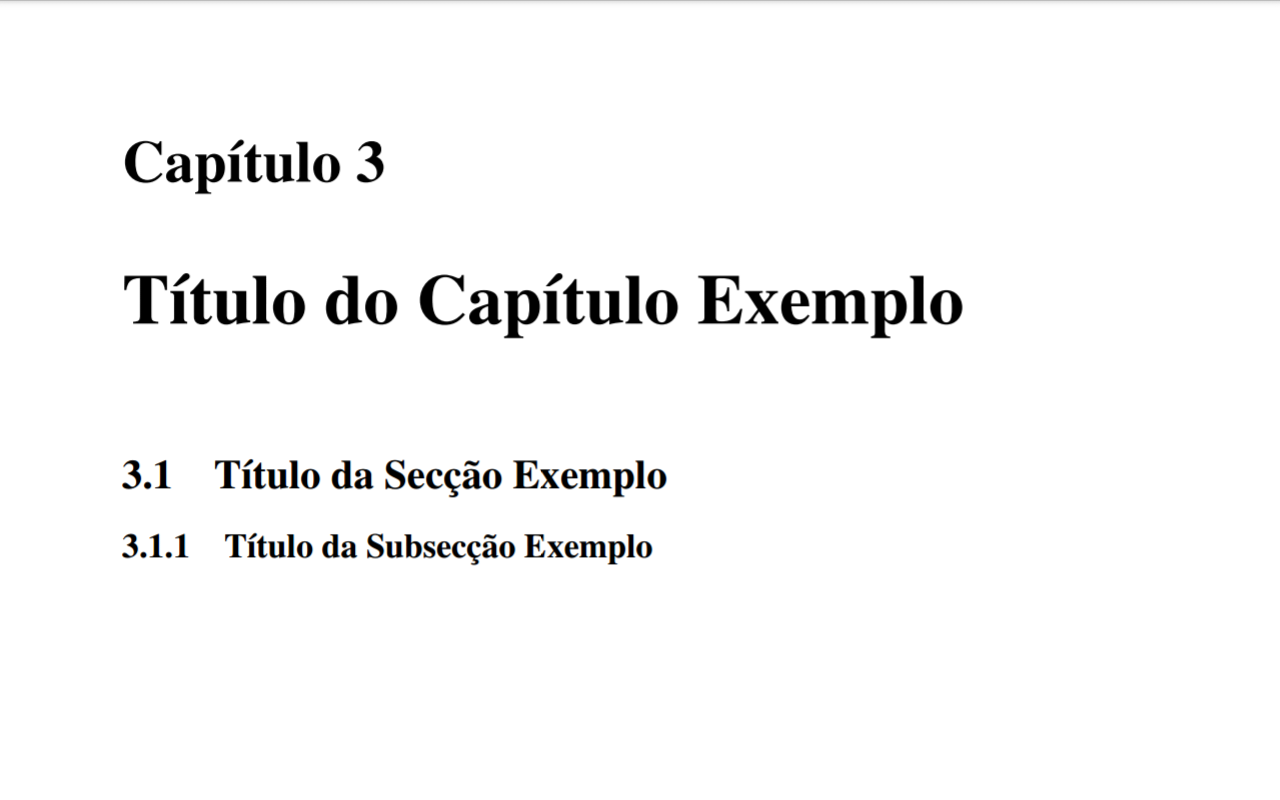
\includegraphics[scale=0.25]{hierarquia}
\caption{Hierarquia gerada pelo código exemplo}
\end{figure}
\flushleft

Como se pode ver, a hierarquia é bem distinta e apareceu numerada de forma organizada e automática.
Esta funcionalidade simplifica muito todo o processo de organização de um documento.

\subsection{Índice Remissivo}

Tal como a numeração de toda hierarquia, o \LaTeX é capaz de automatizar todo o processo de elaboração de um índice.
Apenas é necessária a introdução de um comando: \color{green} \textbackslash tableofcontents \color{black}.

Alternativamente, este comando pode também ser invocado com várias opções de modo a customizar o índice para obter o formato desejado.

As hierarquia descrita no exemplo da Subsecção \ref{subsec.chap} apareceria num índice automático da seguinte forma:

\vspace{5mm}

\begin{figure}[!h]
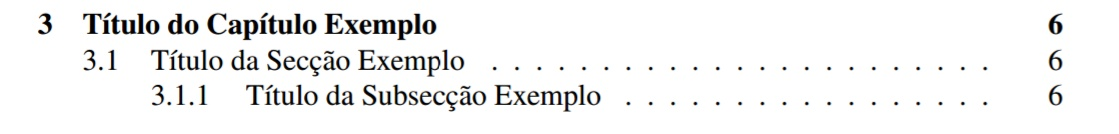
\includegraphics[scale=0.25]{indice}
\caption{Parte de um Índice exemplo}
\end{figure}

\subsection{Lista de figuras / tabelas}

Tal como o que acontece com os capítulos, secções, subsecções e o respetico índice remissivo, o \LaTeX é capaz de numerar automaticamente todas as tabelas e figuras do documento e apresentá-las em forma de lista.
Os comandos para apresentar estas listas são, como no caso do índice, muito simples:


\color{green} \textbackslash listoftables \color{black}, e \color{green} \textbackslash listoffigures \color{black}, respetivamente.


\center
\begin{figure}[!h]
\centering
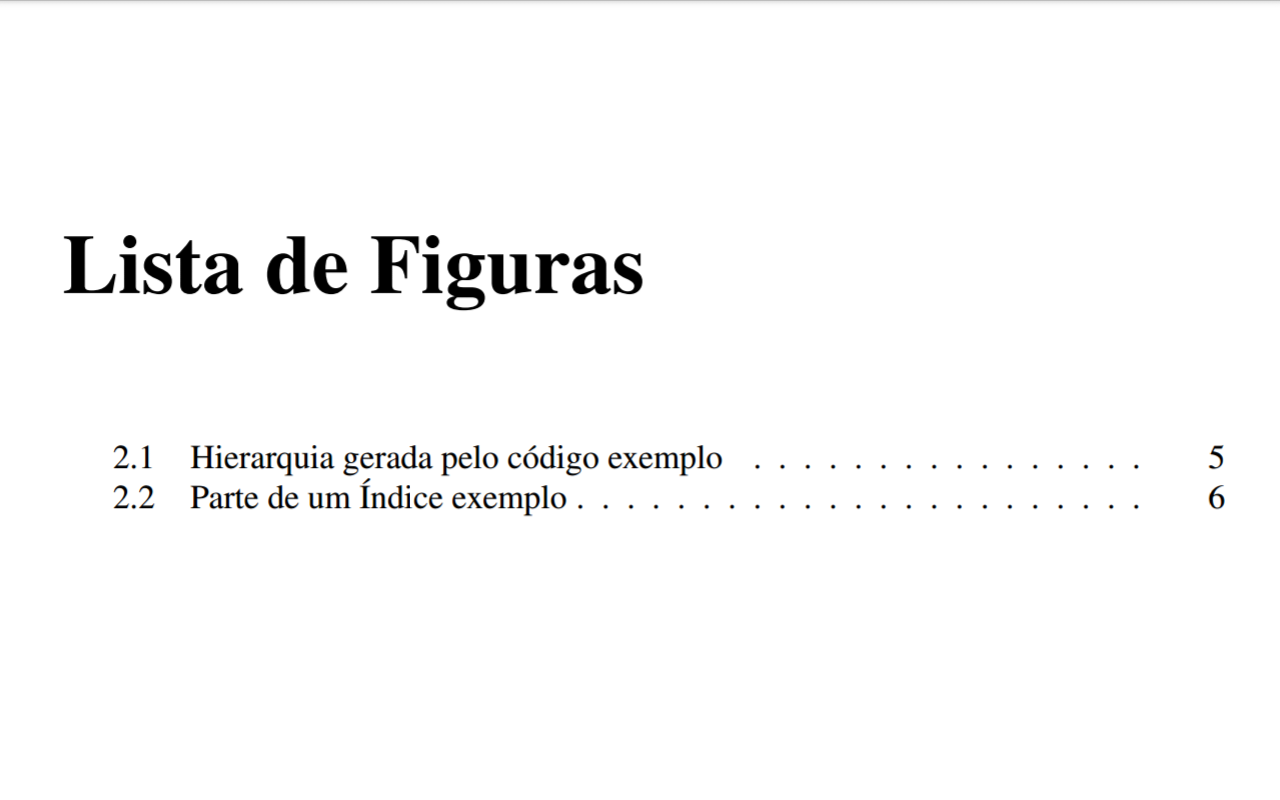
\includegraphics[scale=0.2]{listadefiguras}
\caption{Exemplo de uma lista de figuras gerada automaticamente}
\end{figure}
\flushleft

\subsection{Glossário / Acrónimos}

Ao escrever um documento que contem alguns termos com significado específico é conveniente adicionar ao mesmo um glossário.
O glossário consiste numa lista de termos pouco conhecidos ou específicos de uma certa área, e as suas definições.

Primeiro, é necessário que se invoque a \textbf{package} relevante:

\begin{lstlisting}
\usepackage{glossaries}
\end{lstlisting}

Ou, para o caso de se necessitar de apresentar também uma página semelhante à do glossário mas com o intuito de apresentar as definições de todos os acrónimos utilizados ao longo do documento:

\begin{lstlisting}
\usepackage[acronym]{glossaries}
\end{lstlisting}

Depois, mas ainda antes do comando \color{green} \textbackslash begin\{\color{black}document\color{green}\} \color{black}, deve-se proceder conforme este exemplo:

\begin{lstlisting}
\makeglossaries

\newglossaryentry{termo1}
{
    name=termo1
    description={Descricao do termo 1}
}

\newglossaryentry{termo2}
{
    name=termo2
    description={Descricao do termo 2}
}

\newacronym{ua}{UA}{Universidade de Aveiro}
\newacronym{deti}{DETI}{Departamento de Eletronica, Telecomunicacoes, e Informatica}

\end{lstlisting}

Finalmente, devem ser colocados algures no documento (antes do comando \color{green} \textbackslash end\{ \color{black}document\color{green} \} \color{black}) os comandos:

\begin{lstlisting}
\printglossary[type=\acronymtype] % Apresenta o glossario de acronimos

\printglossary % Apresenta o glossario
\end{lstlisting} ~\cite{glossarios}

\subsection{Bibliografia}

O \LaTeX inclui um suporte de bibliografias compreensivo, com o qual se pode guardar as referências das citações no próprio documento ou num à parte (ficheiro \textbf{.bib}).

Esta funcionalidade é extremamente importante para a eleboração de relatórios sérios que necessitem de citações.

\vspace{5mm}
Exemplo de sintaxe utilizada no ficheiro \textbf{.bib}:

\begin{lstlisting}
@misc{glisc,
	author={{Grey Literature International Steering Committee}},
	title={{GLISC}},
	month={oct},
	year={2014},
	note = "[Online; acedido em Outubro 2014]"
}
\end{lstlisting}

Comandos necessários antes do comando \color{green} \textbackslash begin\{\color{black}document\color{green}\} \color{black}:

\begin{lstlisting}
\usepackage[backend=biber]{biblatex}
\bibliography{nome-do-ficheiro-bib}
\end{lstlisting}

Já no corpo do documento, é possível citar usando:

\begin{lstlisting}
Texto exemplo para demonstracao da funcionalidade de citacao ~\cite{glisc}.
\end{lstlisting}

\begin{figure}[!h]
\centering

\includegraphics[scale=0.2]{biblio}
\caption{Bibliografia gerada pelo código exemplo apresentado}
\end{figure}

Assim, conclui-se que é possivel efetuar citações com o comando \color{green} \textbackslash cite\{\color{black}nome-da-entrada-da-db\color{green} \} \color{black}, desde que exista uma entrada correspondente na base de dados presente no ficheiro \textbf{.bib}
~\cite{bibliografia}

%%%%%%%%%%%%%%%%%%%%%%%%%%%%%%%
\chapter{Manipulação de Texto}
\label{chap.texto}
A escrita em {\LaTeX} permite uma manipulação textual tanto a nível dos caractéres introduzidos, como a nível da estruturação de texto. Estas alterações podem ser uma ser uma simples mudança de cor ou então uma mais complexa alteração na estrutura do texto, como espaçamento entre palavras, criação de listas e/ou tabelas, etc...
\section{Caractéres}
\subsection{Tamanho de Letra}
{\LaTeX} possui uma série de comandos que permitem alterar o tamanho da letra:
 
\begin{lstlisting}
Como {\huge podemos} ver nesta {\tiny pequena} porcao de texto, {\LaTeX} permite-nos {\large alterar} o tamanho de letra a qualquer momento, {\footnotesize sem interrupcoes no texto.}
\end{lstlisting}
 
Como  se {\huge pode} verificar nesta {\tiny pequena} porção de texto, {\LaTeX} permite {\large alterar} o tamanho de letra a qualquer momento, {\footnotesize sem interrupções no texto.}
 
\vspace{4mm}
Aqui está uma lista de comandos para uma alteração do tamanho da letra rápida: ~\cite{guiao}
\begin{itemize}[noitemsep]
	\item \textbackslash tiny
	\item \textbackslash scriptsize
	\item \textbackslash footnotesize
	\item \textbackslash small
	\item \textbackslash normalsize
	\item \textbackslash large
	\item \textbackslash Large
	\item \textbackslash LARGE
	\item \textbackslash huge
	\item \textbackslash Huge
	\item \textbackslash HUGE				
\end{itemize}

Se quiser uma maior liberdade de escolha no tamanho da letra, usando o comando \color{green}\textbackslash fontsize \{\color{black}tamanho\color{green}\} \color{black} pode-se alterar o tamanho da letra para o que pretendemos e com uma maior precisão do que os comandos rápidos em cima apresentados, demonstrado no exemplo seguinte:

\begin{lstlisting}
{\fontsize{50}{60}\selectfont OLA}{\fontsize{5}{6}\selectfont UA!}
{\Huge OLA}{\tiny UA!}
\end{lstlisting} 

\center{\fontsize{50}{60}\selectfont OLÁ}{\fontsize{5}{6}\selectfont UA!}
{\Huge OLÁ}{\tiny UA!}

\vspace{4mm}
\flushleft
\subsection{Fonts}
{\LaTeX} também permite o uso de uma grande variedade de fonts.
Existem 4 famílias diferentes de fonts: ~\cite{fontesSL}
\begin{itemize}
\item \textit{Computer Modern}: Esta família de fonts é a utilizada por defeito em {\LaTeX}
	\begin{itemize}
	\item {\fontfamily{crm}\selectfont CM Roman}
	\item {\fontfamily{cmss}\selectfont CM Sans Serif}
	\item {\fontfamily{cmtt}\selectfont CM Typewriter}
	\end{itemize}
\item \textit{Latin Modern}:
	\begin{itemize}
	\item {\fontfamily{lmr}\selectfont LM Roman}
	\item {\fontfamily{lmss}\selectfont LM Sans Serif}
	\item {\fontfamily{lmtt}\selectfont LM Typewriter}
	\item {\fontfamily{lmdh}\selectfont LM Dunhill}
	\end{itemize}
\item \textit{Post Script Fonts}:
	\begin{itemize}
	\item {\fontfamily{ptm}\selectfont Times}
	\item {\fontfamily{put}\selectfont Utopia/Fourier}
	\item {\fontfamily{ppl}\selectfont Palatino}
	\item {\fontfamily{pbk}\selectfont Bookman}
	\item {\fontfamily{bch}\selectfont Charter}
	\item {\fontfamily{phv}\selectfont Helvetica}
	\item {\fontfamily{pcr}\selectfont Courier}
	\end{itemize}
\item \textit{{\TeX} Gyre}
\end{itemize}
A escolha de font depnde do utilizador. Se a font for necessária para todo o documento, utiliza-se o comando \color{green}\textbackslash usepackage\{\color{black}nome da font\color{green}\}\color{black}. Ao ser ativado este comando, todo o documento irá utilizar a font escolhida. Se não houver qualquer alteração da font, a família de fonts \textit{Computer Modern} é usada como predefinição. Todas as fonts têm um nome definido para poder serem usadas no pacote.

\vspace{4mm}
No entanto, se o utilizador apenas quiser mudar a font do documento apenas temporariamente, deverá utilizar o comando \color{green}\{\textbackslash fontfamily\{\color{black}código da font\color{green}\}\textbackslash selectfont \color{black} texto pretendido\color{green}\}\color{black}. O "código" de uma font é diferente do "nome" mencionado em cima, para ser utilizado no pacote. ~\cite{fontesSL}

\vspace{2mm} 
Por exemplo, a font \textit{Latin Modern Roman} utiliza o nome de pacote \textit{"lmodern"}, enquanto que o seu código é \textit{"lmr"}. Mais destes exemplos encontram-se no link apresentado (Tópico 3 da página: \textit{Reference Guide}). \url{https://www.sharelatex.com/learn/Font_typefaces#!#Reference_guide}

\subsection{Cor}
{\LaTeX} possui várias funcionalidades relacionadas com a cor, desde o texto até à própria página. Para fazer quaiqueres mudanças de cor ao documento, é necessário inicializar o pacote de cor, utilizando o comando \color{green}\textbackslash usepackage\{\color{black}color\color{green}\}\color{black}, (qualquer cor a ser usada posteriormente pelo utilizador não é especificada neste momento).

\vspace{4mm}
Para alterar a cor do texto utiliza-se o código \color{green} \textbackslash color \{\color{black} cor (em inglês) pretendida\color{green} \} \color{black}. Deve-se ter em atenção o facto de que depois de introduzido o comando, todo o texto será transcrito nessa cor. Para voltar à cor inicial usa-se o mesmo comando mas denominando a cor (em inglês novamente) inical do documento. ~\cite{cores}

\vspace{4mm}
\begin{lstlisting}
O texto produzido por este codigo \color{red} ira mudar de vermelho, \color{green} para verde, \color{black} e de volta para a cor inicial.
\end{lstlisting}

\vspace{2mm}
O texto produzido por este código \color{red} irá mudar de vermelho, \color{green} para verde, \color{black} e de volta para a cor inicial.

\vspace{4mm}
{\LaTeX} também permite ao utilizador enfatizar palavras com \colorbox{green}{caixas coloridas}.
Isto pode ser conseguido atráves do código \color{green} \textbackslash colorbox\{\color{black}cor (em inglês) pretendida\color{green}\}\color{black} seguido do texto que se pretende demarcar, \{delimitado por chavetas\}. ~\cite{cores}

\begin{lstlisting}
\colorbox{green}{Esta porcao de texto estara envolvida numa caixa verde.}
\colorbox{green}{\color{orange}Enquanto que esta estara envolvida numa caixa da mesma cor, mas o texto tera uma cor diferente.}

\end{lstlisting}

\vspace{3mm}
\colorbox{green}{Esta porção de texto estará envolvida numa caixa verde.}
\colorbox{green}{\color{orange}Enquanto que esta estará envolvida numa caixa da mesma cor, mas o texto terá uma cor diferente.}

\vspace{2mm}
Como no exemplo, podemos alterar a cor da letra dentro de uma específica caixa, utilizando o comando de cor em cima mencionado. No entanto, não é possível mudar de linha no texto contido dentro de uma caixa de cor. Para isso é necessário abrir uma caixa de cor semelhante, como no exemplo em cima.

\vspace{4mm}
Depois de inicializada a package de cores que em cima foi apresentada, {\LaTeX} passsa a possuir uma palete de cores bastante básica (preto, branco, vermelho, verde, etc...).
Para uma mais vaste gama de cores, é necessário inicializar um outro package, \color{green} \textbackslash usepackage\color{lime} \small[dvipsnames\small]\color{green}\{\color{black}xcolor\color{green}\}\color{black}. Este substituirá aquele inicialmente mencionado.
Este package dá uma maior liberdade de escolha de cores ao utilizador.

Mas {\LaTeX} ainda proporciona uma maior customização de cores. O utilizador poderá definir as suas próprias cores, utilizando o comando \color{green}\textbackslash definecolor\{\color{black}nome\color{green}\}\{\color{black}modelo\color{green}\}\{\color{black}espectro\color{green}\}\color{black}, onde: ~\cite{cores}
\begin{itemize}
\item o "nome" é a denominação da cor à escolha do utilizador
\item o "modelo" é a \textit{descrição} da cor, e pode ser:
	\begin{itemize}
	\item gray - escala de cinzentos de 0 (preto) a 1 (branco);
	\item rgb - palete de cores \textit{RED GREEN BLUE} definida por 3 números de 0 a 1;
	\item RGB - gama de cores \textit{RED GREEN BLUE} representado por 3 números de 0 a 255;
	\item HTML - seis valores hexadecimais são atribuídos numa forma \textit{RRGGBB};
	\item cmyk - palete de cores \textit{Ciano, Magenta, Amarelo, Preto}, em que é atribuído um valor de 0 a 1 a cada uma dessas cores;
	\end{itemize}
\item o "espectro" são os valores dados pelo utilizador para criar a cor. Estes valores terão de estar de acordo com os valores válidos para cada modelo e, no caso de existência de vários valores, serão separados por vírgulas.
\end{itemize}

Por exemplo, com o código... ~\cite{cores}
\begin{lstlisting}
\definecolor{cinzento-claro}{gray}{0.50}
\end{lstlisting}
\definecolor{cinzento-claro}{gray}{0.50}
Ficará para futura utilização uma cor denominada "cinzento-claro", \color{cinzento-claro}com este aspeto\color{black}.

A cor definida ficará gravada no documento e para ser utilizada será apenas necessário o comando de cor, completo com o nome da criação do utilizador.

Para descobrir a lista completa de cores que se poderá utilizar e mais exemplos de criação de cores como apresentado em cima, consulte a página de web contida no link seguinte.

\url{https://en.wikibooks.org/wiki/LaTeX/Colors}

A informação revlevante ao assunto encontra-se nos tópicos 4 e 5 da página.

\subsection{Outras Tranformações}
{\LaTeX	} também consegue realizar pequenas transformações de texto como \textbf{negrito}, \textit{itálico}, etc..., através de simples comandos.
\subsubsection{Negrito}
Para colocarmos o texto a negrito utiliza-se o simples comando \color{green} \textbackslash textbf \color{black} e denominar o texto que se quer a negrito \{dentro de chavetas\}. ~\cite{fontesWB}

Exemplo:
\begin{lstlisting}
\textbf{Este texto aparecera a negrito}, enquanto que este nao.
\end{lstlisting}
\textbf{Este texto aparecerá a negrito}, enquanto que este não.

\subsubsection{Itálico}
Texto em itálico é também simples, tal como negrito. O código
\color{green}\textbackslash textit \color{black} irá tranformar o texto contido \{dentro de chavetas\} em itálico.  ~\cite{fontesWB}

Exemplo:
\begin{lstlisting}
\textit{Este texto aparecera em italico}, enquanto que este nao.
\end{lstlisting}
\textit{Este texto aparecerá em italico}, enquanto que este não.

\subsubsection{Sublinhar Texto}
{\LaTeX} também consegue sublinhar texto, isto através do código \color{green} \textbackslash underline \color{black}, seguido do texto que se pretende sublinhar, \{delimitado por chavetas\}. ~\cite{fontesWB}

Exemplo:
\begin{lstlisting}
\underline{Este texto aparecera sublinhado}, enquanto que este nao.
\end{lstlisting}
\underline{Este texto aparecerá sublinhado}, enquanto que este não.

\subsubsection{Ênfase}
A ênfase de texto funciona com o código \color{green} \textbackslash emph \color{black}, seguido do texto que se pretende enfatizar, sempre \{delimitado por chavetas\}. ~\cite{fontesWB}

Exemplo:
\begin{lstlisting}
Nesta porcao de texto o comando para enfatizar tornara o texto em \emph{italico}.
\textit{Enquanto que nesta, o comando faz com que o texto \emph{deixe de estar} em italico}.
\end{lstlisting}

Nesta porção de texto o comando para enfatizar tornará o texto em \emph{itálico}.
\textit{Enquanto que nesta, o comando faz com que o texto \emph{deixe de estar} em itálico}.

\vspace{4mm}
Como verificado no exemplo acima, o comando de enfatização altera o texto da sua forma definida como norma. Se o texto se encontrar normal, este tornará a porção de texto pretendida em itálico. Se o texto já se encontrar em itálico, o comando irá normalizar o texto \{delimitado por chavetas\}.

\section{Formatação}
Relativamente à estruturação de texto, {\LaTeX} oferece uma grande customização. Desde a formatação de paragráfos até à criação de notas de rodapé, tudo pode ser conseguido com os certos comandos.

A formatação de texto em {\LaTeX} é muito customizável, chegando até a ser excessivo. Isto cria um certo grau de dificuldade nesta área. No entanto, o resultado final do texto formatado mostra que o elevado cuidado e atenção à formatação, elevam o documento a outro nível de profissionalismo.
\subsection{Parágrafos}
Parágrafos podem ser definidos na raiz do domcumento antes de se ter começado a redigir. Isto significa que alguns comandos terão de ser inicializados tal como uma package.
São 3 os comandos essenciais para a formatação de parágrafos:
\begin{enumerate}
\item \color{green} \textbackslash setlenght \{\textbackslash parindent\}\{\color{black} valor\color{green}\}\color{black};
	\begin{itemize}
	\item Este comando seleciona o comprimento desde a Margem da página até ao início do parágrafo;
	\item O valor vem normalmente em unidades \textit{"em"} que é a distância que um "M" maiúsculo na font definida ocupa. Ou seja, \textit{4em} ocupa um espaço equivalente a "MMMM".
	\end{itemize}
\item \color{green} \textbackslash setlenght \{\textbackslash parskip\}\{\color{black} valor\color{green}\}\color{black};
	\begin{itemize}
	\item Este comando define o espaço entre cada parágrafo, quando um é introduzido;
	\item O valor vem também em unidades \textit{"em"}.
	\end{itemize}
\item \color{green} \textbackslash renewcommand \{\textbackslash baselinestretch\}\{\color{black} valor\color{green}\}\color{black}.
	\begin{itemize}
	\item Este comando define o espaçamento entre as linhas do documento;
	\item Este valor pode ser qualquer número.
	\end{itemize}
\end{enumerate}

Todos este comandos são, normalmente, inicializados junto dos packages, no entanto, o utilizador poderá querer usar ou definir diferentes tamanhos para qualquer um dos parâmetros numa certa localização do documento. Para isso, basta reescrever o(s) comando(s) no local desejado. ~\cite{paragrafos}

\subsection{\textit{Breaks}}

\begin{itemize}
\item Linhas 
	\begin{itemize}
	\item \textit{Breaks} de linhas são utilizados para mudar de linha sem que esta faça a marca de parágrafo automaticamente; ~\cite{paragrafos}
	\item Isto é feito através da colocação de -\color{green} \textbackslash\textbackslash \color{black} ou \color{green}\textbackslash newline \color{black} - no final da linha que queremos terminar. ~\cite{paragrafos}
	\end{itemize}
\item Páginas
	\begin{itemize}
		\item Tal como os \textit{Breaks} de linhas, mas covertidos para páginas, estes \textit{Breaks} fazem com que o documento mude para a seguinte página, deixando o resto da página corrente em branco. ~\cite{espacos}
		\item Isto é conseguido através do código \color{green}\textbackslash clearpage \color{black} ~\cite{espacos}
	\end{itemize}
\end{itemize}

\subsection{Preenchimento de Linhas}
\begin{itemize}
\item Preenchimento Horizontal ~\cite{espacos}
	\begin{itemize}
	\item O preenchimento horizontal de linhas coloca um espaço em branco da maneira que o utilizador desejar;
	\item O comando \color{green} \textbackslash hspace\{\color{black}valor\color{green}\}\color{black} preenche horizontalmente com um espaço em branco do tamanho do valor introduzido pelo redator (este valor pode ser escrito em qualquer unidade suportada por {\LaTeX});
	\item O comando \color{green} \textbackslash hfill \color{black} preenche com um espaço em branco, também horizontalmente, o restante espaço não ocupado na linha;
	\end{itemize}
\item Preenchimento Vertical ~\cite{espacos}
	\begin{itemize}
	\item Tal como o preenchimento horizontal, o vertical tem a mesma função, mas em sentido oposto;
	\item Para um preenchimento da linha não automatizado, usa-se o comando \color{green} \textbackslash vspace\{\color{black}valor\color{green}\}\color{black}em que o valor também pode ser em qualquer unidade suportada por {\LaTeX};
	\item para um preenchimento vertical automático utiliza-se o comando \color{green} \textbackslash vfill \color{black};
	\end{itemize}
\end{itemize}

\subsection{Alinhamento Textual}
Para o alinhamento de texto, {\LaTeX} possui um conjunto de comandos que permite uma estruturação bem definida. No entanto a package \textit{ragged2e} dá outro ambiente aos comandos de alinhamento e, também muito importante, faz com que hífens possam ser justificados e alinhados corretamente.
Para isto, é necessário iniciar a package, com o comando \color{green}\textbackslash usepackage\{\color{black}ragged2e\color{green}\}\color{black}. ~\cite{paragrafos}

\subsubsection{Alinhamento à Esquerda}
O comando para uma justificação à esquerda, utilizando o ambiente \textit{ragged2e} é \color{green}\textbackslash FlushLeft \color{black}.
Para utilizar uma justificação à esquerda para todo o documento utiliza-se um comando \textit{switch}, que depois de ativado, apenas é desativado com um outro comando tipo \textit{switch}. Isto é útil para grande blocos de texto ou o documento intiero.
Neste caso o comando é \color{green} \textbackslash RaggedRight \color{black} (NOTA: Apesar de contra-intuitivo, este é o código correto!). ~\cite{paragrafos}

\subsubsection{Alinhamento à Direita}
O comando para uma justificação à direita, é \color{green}\textbackslash FlushRight \color{black}.
Utilizando novamente o comando \textit{switch}, mas desta vez, destinado a uma justificação à direita.
Neste caso o comando é \color{green} \textbackslash RaggedLeft \color{black} (NOTA: O mesmo acontece com este comando!). ~\cite{paragrafos}

\subsubsection{Alinhamento ao Centro}
O comando para uma justificação ao centro, é \color{green}\textbackslash Center \color{black}.
Novamente, tal como nos dois casos prévios existem comandos \textit{switch }.
Neste caso o comando é \color{green} \textbackslash RaggedLeft \color{black} (NOTA: O mesmo acontece com este comando!). ~\cite{paragrafos}

\subsubsection{Justificação Total}
O ambiente \textit{ragged2e} também possúi um método de total justificação do documento. Isto é possível através do código \color{green} \textbackslash justify \color{black}. ~\cite{paragrafos}

\vfill
\subsection{Notas de Rodapé}
Por vezes, em alguns documentos é necessário a utilização de notas de rodapé\footnote{Por vezes são úteis}... Estas também podem ser criadas em {\LaTeX }.
Para isto usamos o comando \color{green} \textbackslash footnote\color{lime}[número de nota]\color{green}\{\color{black} nota a acrescentar\color{green}\}\color{black}.

Ao ler o ficheiro \textbf{.tex} ter as notas próximas do texto principal pode mostrar-se um pouco confuso. Para não ocorrer esse problema usa-se o comando \color{green} \textbackslash footnotemark \color{black}. Este comando marca uma nota de roda pé. Para mais tarde aceder a essa nota usa-se o comando \color{green} \textbackslash footnotetext\{\color{black} nota a acrescentar\color{green}\}\color{black}. Este comando pode ser colocado em qualquer lado do documento \textbf{.tex}. Isto desde que mais nenhuma nota de roda pá tenha sido ainda marcada.

Podemos\footnotemark também utilizar várias referências\footnotemark[\value{footnote}] para a mesma nota. Isto pode ser feito adicionando ao comando de marcação de nota, em cima mencionado, o comando \color{green} \textbackslash footnotemark\color{lime}[\textbackslash value \color{green}\{\color{black}footnote\color{green}\}\color{lime}]\color{black}. Este comando utiliza o valor da nota de rodapé marcada e reutiliza-o. També é possível utilizar o comando \color{green} \textbackslash footnotetext\{\color{black} nota a acrescentar\color{green}\}\color{black} neste caso. ~\cite{rodape}

\footnotetext{Este nota tem duas referências}




\chapter{Escrita de fórmulas matemáticas}
\label{chap.mat}
Uma das funcionalidades mais atrativas do \LaTeX para a comunidade científica é a escrita de fórmulas matemáticas complexas de forma fácil e com apresentação correta. É especialmente útil para fórmulas com contenham símbolos pouco usados no dia-a-dia.

Equações básicas em \LaTeX são fácilmente 'programáveis', como se pode ver no exemplo seguinte (Teorema de Pitágoras): ~\cite{matematica}

\begin{lstlisting}
\[ x^2 + y^2 = z^2 \]
\end{lstlisting}

\[ x^2 + y^2 = z^2 \]

No entanto, a forma mais correta de incluir fórmulas num documentto é usando o modo de matemática.

\section{Modo de matemática}

O \LaTeX permite a escrita de fórmulas matemáticas em dois modos distintos. Estes são o modo \textbf{inline}\footnote{\textbf{inline} - na própria linha}, e o modo \textbf{display}\footnote{\textbf{display} - destacado do resto }. A diferença entre eles pode ser verificada no exemplo seguinte: ~\cite{matematica}

\begin{lstlisting}
% Modo inline: 
A equivalencia massa-energia e descrita pela famosa equacao $E=mc^2$, descoberta em 1905 por Albert Einstein.

% Modo display: 
A equivalencia massa-energia e descrita pela famosa equacao $$E=mc^2$$, descoberta em 1905 por Albert Einstein.
\end{lstlisting} 

A equivalência massa-energia é descrita pela famosa equação $E=mc^2$, descoberta em 1905 por Albert Einstein.

\vspace{5mm}
A equivalência massa-energia é descrita pela famosa equação $$E=mc^2$$ descoberta em 1905 por Albert Einstein.

\vspace{3mm}
\rule{12cm}{0.4pt}
\vspace{3mm}

Para utlizar o modo \textbf{inline}, podem ser usados um dos seguintes conjuntos de delimitadores:  ~\cite{matematica}

\begin{center}
\textbackslash ( ... \textbackslash ), \$ ... \$, \textbackslash begin\{math\} ... \textbackslash end\{math\}
\end{center}

\vspace{5mm}

Para utlizar o modo \textbf{display}, podem ser usados um dos seguintes conjuntos de delimitadores:  ~\cite{matematica}

\begin{center}
\textbackslash [ ... \textbackslash ], \$\$ ... \$\$, \textbackslash begin\{displaymath\} ... \textbackslash end\{displaymath\}\footnote{Em vez de \textbf{displaymath}, também se pode usar \textbf{equation}.}
\end{center}

Como já foi possível verificar, o símbolo '\^' serve, no modo matemático do \LaTeX, para escrever expoentes em equações. 
Existe outro carater especial digno de referência, '\_'. Este tem o propósito de indicar um índice. ~\cite{guiao}

\section{Símbolos matemáticos}
Alguns exemplos de símbolos matemáticos incluídos no \LaTeX podem ser encontrados nas tabelas que se seguem:

\begin{table}[!h]
\centering
\begin{tabular}{|l|l|l|l|}
%
\hline
\color{green} \textbackslash alpha A \color{black} & $\alpha A$ & \color{green} \textbackslash nu N \color{black} & $\nu N$ \\ \hline
\color{green} \textbackslash beta B \color{black} & $\beta B$ & \color{green} \textbackslash xi \textbackslash Xi \color{black} & $\xi \Xi$ \\ \hline
\color{green} \textbackslash gamma \textbackslash Gamma \color{black} & $\gamma \Gamma$ & \color{green} o O \color{black} & $o O$ \\ \hline
\color{green} \textbackslash delta \textbackslash Delta \color{black} & $\delta \Delta$ & \color{green} \textbackslash pi \textbackslash Pi \color{black} & $\pi \Pi$ \\ \hline
\color{green} \textbackslash epsilon \textbackslash varepsilon E \color{black} & $\epsilon \varepsilon E$ & \color{green} \textbackslash rho \textbackslash varrho P\color{black} & $\rho \varrho P$ \\ \hline
\color{green} \textbackslash zeta Z \color{black} & $\zeta Z$ & \color{green} \textbackslash sigma \textbackslash Sigma \color{black} & $\sigma \Sigma$ \\ \hline
\color{green} \textbackslash eta H \color{black} & $\eta H$ & \color{green} \textbackslash tau T \color{black} & $\tau T$ \\ \hline
\color{green} \textbackslash theta \textbackslash vartheta \textbackslash Theta \color{black} & $\theta \vartheta \Theta$ & \color{green} \textbackslash upsilon \textbackslash Upsilon \color{black} & $\upsilon \Upsilon$ \\ \hline 
\color{green} \textbackslash iota I \color{black} & $\iota I$ & \color{green} \textbackslash phi \textbackslash varphi \textbackslash Phi \color{black} & $\phi \varphi \Phi$ \\ \hline
\color{green} \textbackslash kappa K \color{black} & $\kappa K$ & \color{green} \textbackslash chi X \color{black} & $\chi X$ \\ \hline
\color{green} \textbackslash lambda \textbackslash Lambda \color{black} & $\lambda \Lambda$ & \color{green} \textbackslash psi \textbackslash Psi \color{black} & $\psi \Psi$ \\ \hline
\color{green} \textbackslash mu M \color{black} & $\mu M$ & \color{green} \textbackslash omega \textbackslash Omega \color{black} & $\omega \Omega$ \\ \hline
%
\end{tabular}
\caption{Exemplos de símbolos gregos (para usar em equações) ~\cite{simbolos}}
\end{table}

\begin{table}[!h]
\centering
\begin{tabular}{|l|l|l|l|}
%
\hline
\color{green} \textbackslash infty \color{black} & $\infty$ & \color{green} \textbackslash forall \color{black} & $\forall$ \\ \hline
\color{green} \textbackslash Re \color{black} & $\Re$ & \color{green} \textbackslash Im \color{black} & $\Im$ \\ \hline
\color{green} \textbackslash nabla \color{black} & $\nabla$ & \color{green} exists \color{black} & $\exists$ \\ \hline
\color{green} \textbackslash partial \color{black} & $\partial$ & \color{green} \textbackslash emptyset \color{black} & $\emptyset$ \\ \hline
\color{green} \textbackslash times \color{black} & $\times$ & \color{green} \textbackslash div \color{black} & $\div$ \\ \hline
\color{green} \textbackslash cap \color{black} & $\cap$ & \color{green} \textbackslash cup \color{black} & $\cup$ \\ \hline
\color{green} \textbackslash neq \color{black} & $\neq$ & \color{green} \textbackslash subset \color{black} & $\subset$ \\ \hline 
\color{green} \textbackslash leq \color{black} & $\leq$ & \color{green} \textbackslash geq \color{black} & $\geq$ \\ \hline
\color{green} \textbackslash in \color{black} & $\in$ & \color{green} \textbackslash notin \color{black} & $\notin$ \\ \hline
\color{green} \textbackslash wedge \color{black} & $\wedge$ & \color{green} \textbackslash vee \color{black} & $\vee$ \\ \hline
\color{green} \textbackslash simeq \color{black} & $\simeq$ & \color{green} \textbackslash approx \color{black} & $\approx$ \\ \hline
\color{green} \textbackslash equiv \color{black} & $\equiv$ & \color{green} \textbackslash cong \color{black} & $\cong$ \\ \hline
%
\end{tabular}
\caption{Exemplos de símbolos matemáticos avulsos (para usar em equações) ~\cite{simbolos}}
\end{table}


\chapter{Listas, Tabelas e Imagens}
\label{chap.listas,tabelas e imagens}
{\LaTeX}, como sistema de preparação de texto, possúi também maneiras para criar listas, tabelas e gráficos. E tal como todas as outras funcionalidades, estas também estão munidas de um elevado grau de customização.

\section{Listas}
A criação de listas é uma tarefa bastante intuitiva. O exemplo abaixo demonstra isso: ~\cite{guiao}
\begin{lstlisting}
\begin{itemize}
	\item Este e o 1o elemento de uma lista
	\item Este e o 2o elemento da mesma lista
\end{itemize}
\end{lstlisting}
\begin{itemize}
	\item Este é o 1º elemento de uma lista
	\item Este é o 2º elemento da mesma lista
\end{itemize}

\vspace{2mm}
Como se pode verificar a criação de listas é uma tarefa simples. Mas um elevado número de pequenos detalhes de código que pode ser adicionadas às listas, faz com que estas sejam muito customizáveis. Como no exemplo em baixo, no qual é necessário a invocação de uma nova package, com o comando \color{green}\textbackslash usepackage\{\color{black}enuitem\color{green}\}\color{black}. 
\begin{lstlisting}
\begin{itemize}[noitemsep]
	\item Estes items 
	\item Terao um diferente espacamento
	\item Dos items do exemplo dado em cima
\end{itemize}
\end{lstlisting}
\begin{itemize}[noitemsep]
	\item Estes items 
	\item Terão um diferente espaçamento
	\item Dos items do exemplo dado em cima
\end{itemize}

\clearpage
Também é possível a criação de listas horizontais. É, no entanto, necessário a inicialização de uma nova package para que isso seja possível, com o comando \color{green}\textbackslash usepackage\{\color{black}tasks\color{green}\}\color{black}. Posteriormente, em vez do código \textit{itemize} é usado o código \textit{task}.

\vspace{5mm}
Também é possível colocar listas dentro de um item de uma outra lista ~\cite{guiao}

\begin{lstlisting}
\begin{itemize}
	\item Este e o 1o item de uma lista
	\begin{itemize}
		\item Este e o 1o elemento de uma lista secundaria
		\item Estes items estao contidos no 1o item da 1a lista
	\end{itemize}
	\item Este e o 2o item da 1a lista
\end{itemize}
\end{lstlisting}
\begin{itemize}
	\item Este é o 1º item de uma lista
	\begin{itemize}
		\item Este é o 1º elemento de uma lista secundária
		\item Estes items estão contidos no 1º item da 1ª lista
	\end{itemize}
	\item Este é o 2º item da 1ª lista
\end{itemize}

\vspace{3mm}
Os elementos de uma lista também podem ser numerados. Estes items também podem conter uma lista numerada dentro de s, como no exemplo dado em cima. Em vez da utilização do código \textit{itemize}, é colocado \{dentro das chavetas\} o código \textit{enumerate}. ~\cite{guiao}

\begin{lstlisting}
\begin{enumerate}
	\item Este e o 1o item de uma lista
	\begin{enumerate}
	
	\end{enumerate}
		\item Este e o 1o elemento de uma lista secundaria
		\item Estes items estao contidos no 1o item da 1a lista
	\end{enumerate}
	\item Este e o 2o item da 1a lista
\end{enumerate}
\end{lstlisting}
\begin{enumerate}
	\item Este é o 1º item de uma lista
	\begin{enumerate}
		\item Este é o 1º elemento de uma lista secundária
		\item Estes items estão contidos no 1º item da 1ª lista
	\end{enumerate}
	\item Este é o 2º item da 1ª lista
\end{enumerate}


\clearpage
\section{Tabelas}
Tabelas podem ser usadas como forma de listagem ou se forem mais complexas, uma ferramenta de comparação ou de fornecimento de informação compacta. {\LaTeX} permite-nos a criação de todo o tipo de tabelas. ~\cite{guiao}

\begin{lstlisting}
\begin{center}
\begin{tabular}{ c c c }
 Elemento 1 & Elemento 4 & Elemento 7 \\ 
 Elemento 2 & Elemento 5 & Elemento 8 \\  
 Elemento 3 & Elemento 6 & Elemento 9    
\end{tabular}
\end{center}
\end{lstlisting}


\begin{center}
\begin{tabular}{ c c c }
 Elemento 1 & Elemento 4 & Elemento 7 \\ 
 Elemento 2 & Elemento 5 & Elemento 8 \\  
 Elemento 3 & Elemento 6 & Elemento 9    
\end{tabular}
\end{center}

\vspace{3mm}
O exemplo acima mostra uma tabela centralizada muito rudimentar.
\begin{lstlisting}
\begin{center}
\begin{tabular}{| c | c | c |}
 \hline	
 Elemento 1 & Elemento 4 & Elemento 7 \\
 \hline
 Elemento 2 & Elemento 5 & Elemento 8 \\
 \hline  
 Elemento 3 & Elemento 6 & Elemento 9 
 \hline   
\end{tabular}
\end{center}
\end{lstlisting}

\begin{center}
\begin{tabular}{| c | c | c |}
 \hline	
 Elemento 1 & Elemento 4 & Elemento 7 \\ 
 \hline
 Elemento 2 & Elemento 5 & Elemento 8 \\
 \hline  
 Elemento 3 & Elemento 6 & Elemento 9 \\
 \hline   
\end{tabular}
\end{center}

No 2º exemplo, verifica-se que a adição de umas pequenas linhas ao código do 1º exemplo, a tabela transforma-se.

Outras modificações simples podem ser feitas substituíndo a letra \textit{c}, que neste código está a centralizar os elementos da tabela, pela letra \textit{l} ou \textit{r} que irão alinhar o texto à esquerda e à direita respetivamente.

O código \color{green}\textbackslash hline \color{black} coloca uma linha horizontal nos limites da tabela. Isto pode ser usado um número ilimitado de vezes.

O símbolo \textit{\&} separa os elementos da tabela e para terminar uma linha na tabela, e delimitar a mesma, usa-se \color{green} \textbackslash\textbackslash\color{black}.
\clearpage ~\cite{tabelas}

Várias alterações podem ser feitas a uma tabela. Os exemplos dados são tabelas simples, porque {\LaTeX} oferece infinitas possibilidades de customização para a criação de tabelas. Isto inclúi combinação de linhas e colunas de tabelas, tabelas de duas ou mais páginas, alterar o aspeto de uma tabela, etc...\\
Mais destas customizações estão disponíveis no link abaixo:
\newline
\url{https://www.sharelatex.com/learn/Tables}

\section{Imagens}
{\LaTeX} Também permite a inserção de imagens. Para tal é necessário a inicialização de uma nova package, usando o código \color{green}\textbackslash usepackage\{\color{black}graphicx\color{green}\}\color{black}.
Como a inserção de imagens invoca um ficheiro de imagem, é necessário indicar o seu \textit{path}\footnote{especificação completa do diretório onde se encontra o ficheiro}. Isso pode ser feito no momento de invocação do ficheiro, mas como alternativa, se todos os ficheiros de imagem estiverem contidos no mesmo diretório, é possível definir o \textit{path} no início do documento, para facilitar a invocação das imagens quando for necessário. Isto é possível através do comando \color{green}\textbackslash graphicspath\{ \{\color{black}\textit{path}/\color{green}\} \}\color{black}. ~\cite{imagens}

\begin{lstlisting}
A imagem abaixo mostra uma vista aerea de parte do campus da Universidade de Aveiro. A imagem foi retirada do site da UA (ua.pt).
\centering
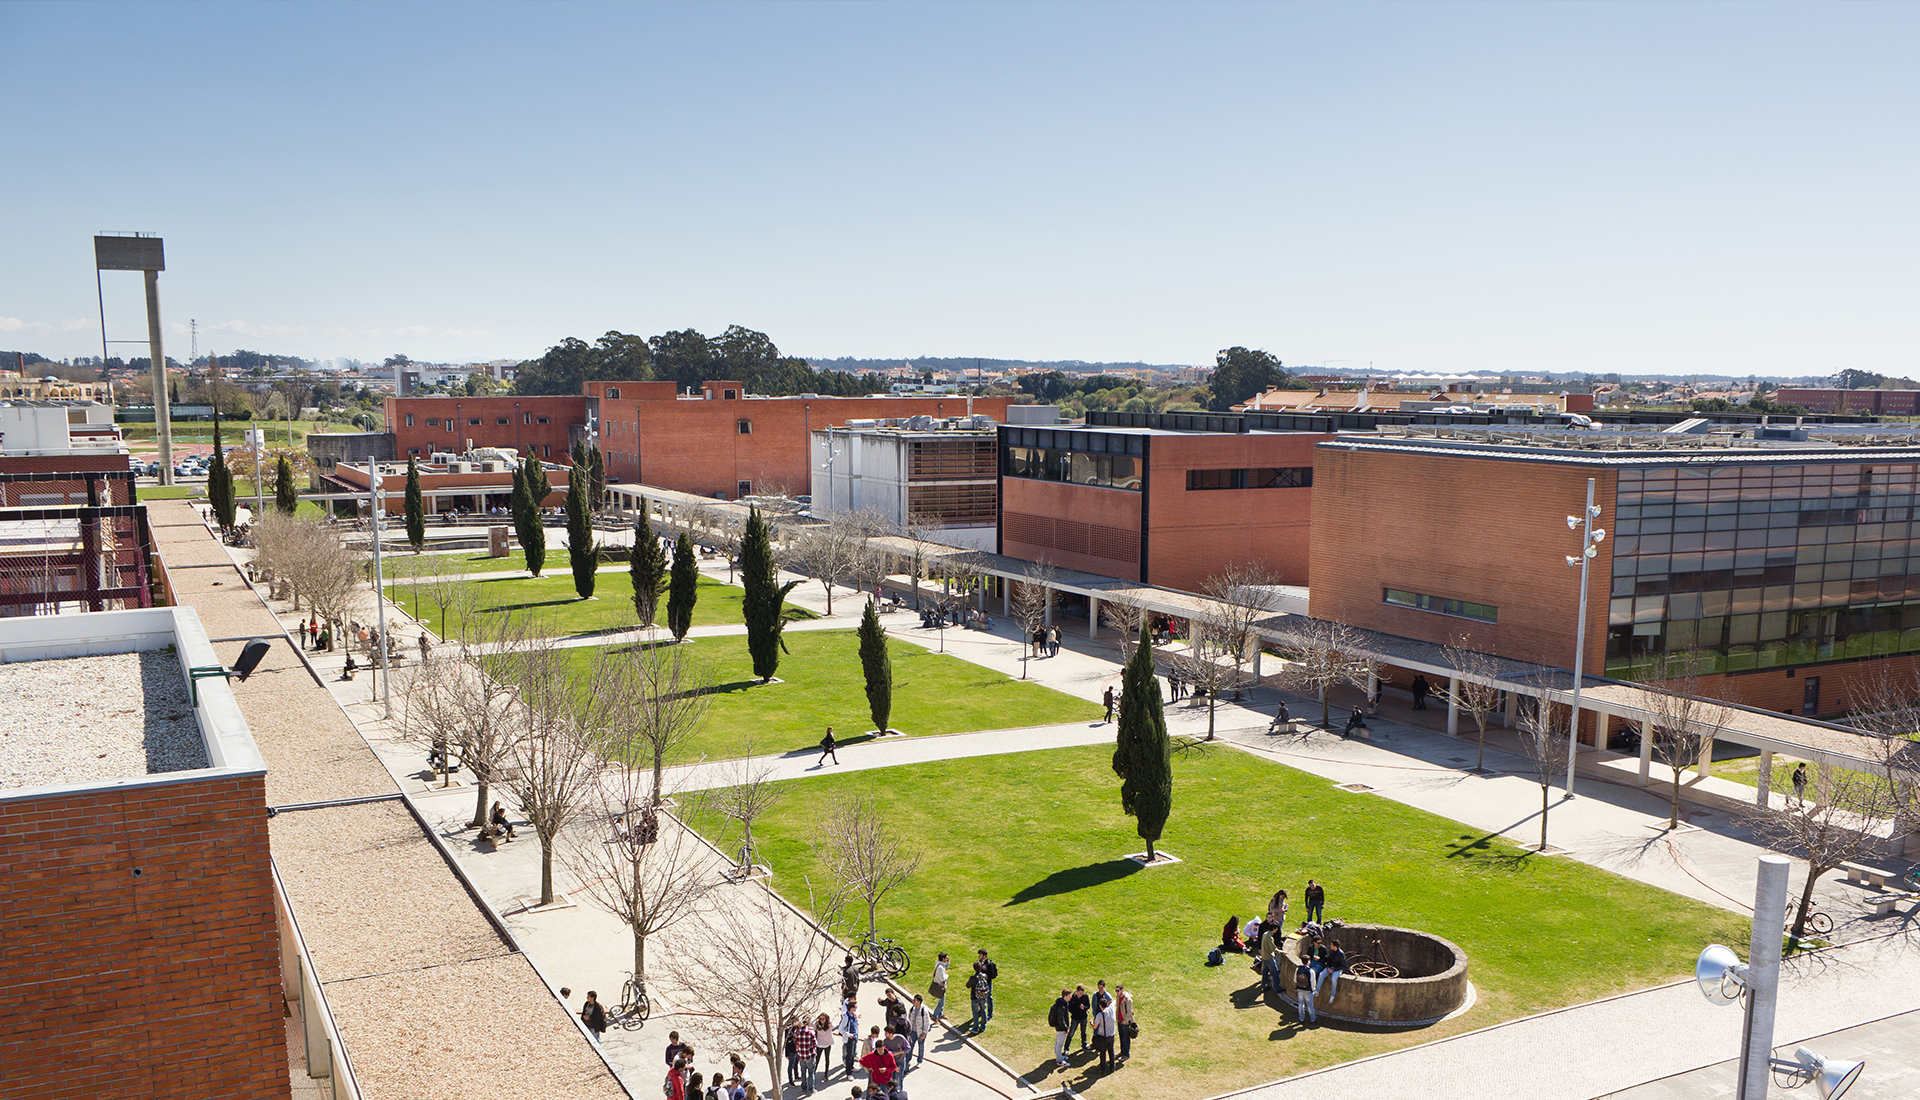
\includegraphics[scale=0.15]{Campus}
\end{lstlisting}

A imagem abaixo mostra uma vista aérea de parte do campus da Universidade de Aveiro. A imagem foi retirada do site da UA (ua.pt).

\vspace{2mm}
\centering
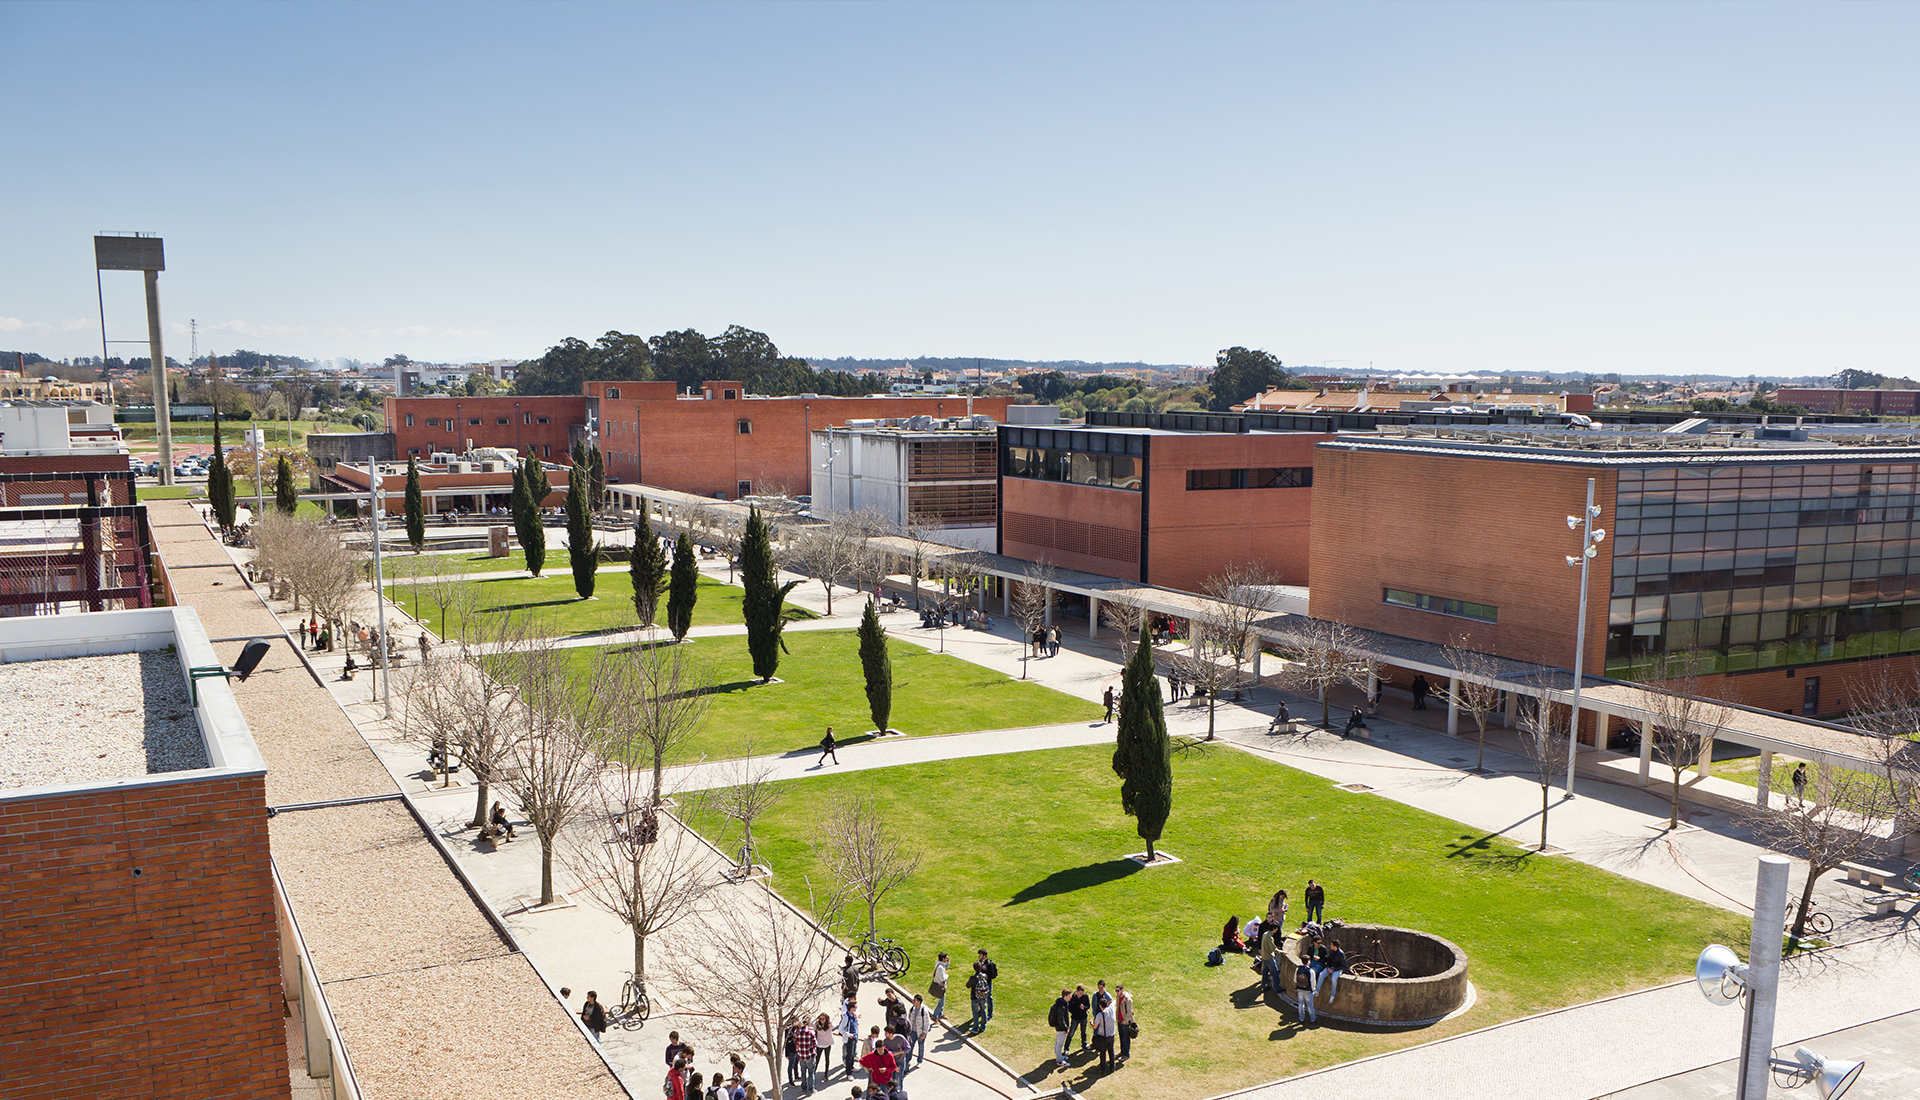
\includegraphics[scale=0.15]{Campus}

\clearpage
\RaggedRight
Como de pode verificar no exemplo acima, para chamar um ficheiro com formato de imagem, é necessário o código \color{green}\textbackslash includegraphics\{\color{black}nome do ficheiro\color{green}\}\color{black}.
Neste caso, como o ficheiro tinha uma dimensão demasiado grande, diminui-se a escala para ficar do tamanha desejado. Isto é possível através da extensão \color{lime}[\color{black}scale=escala pretendida\color{lime}]\color{black}. 

No entanto, também é possível formatar a imagem como o utilizador desejar. Em vez da extensão \textit{scale} usa-se o controlo de largura \textit{widht=xcm} e o controlo de comprimento \textit{height=ycm} e controlo de rotação \textit{angle=z}(\textit{x} e \textit{y} serão valores introduzidos pelo redator do documento, numa unidade qualquer). Isto permite ao utilizador distorcer a imagem como for necessário.  ~\cite{imagens}

\begin{lstlisting}
A imagem utilizada em cima ira agora aparecer distorcida

\centering
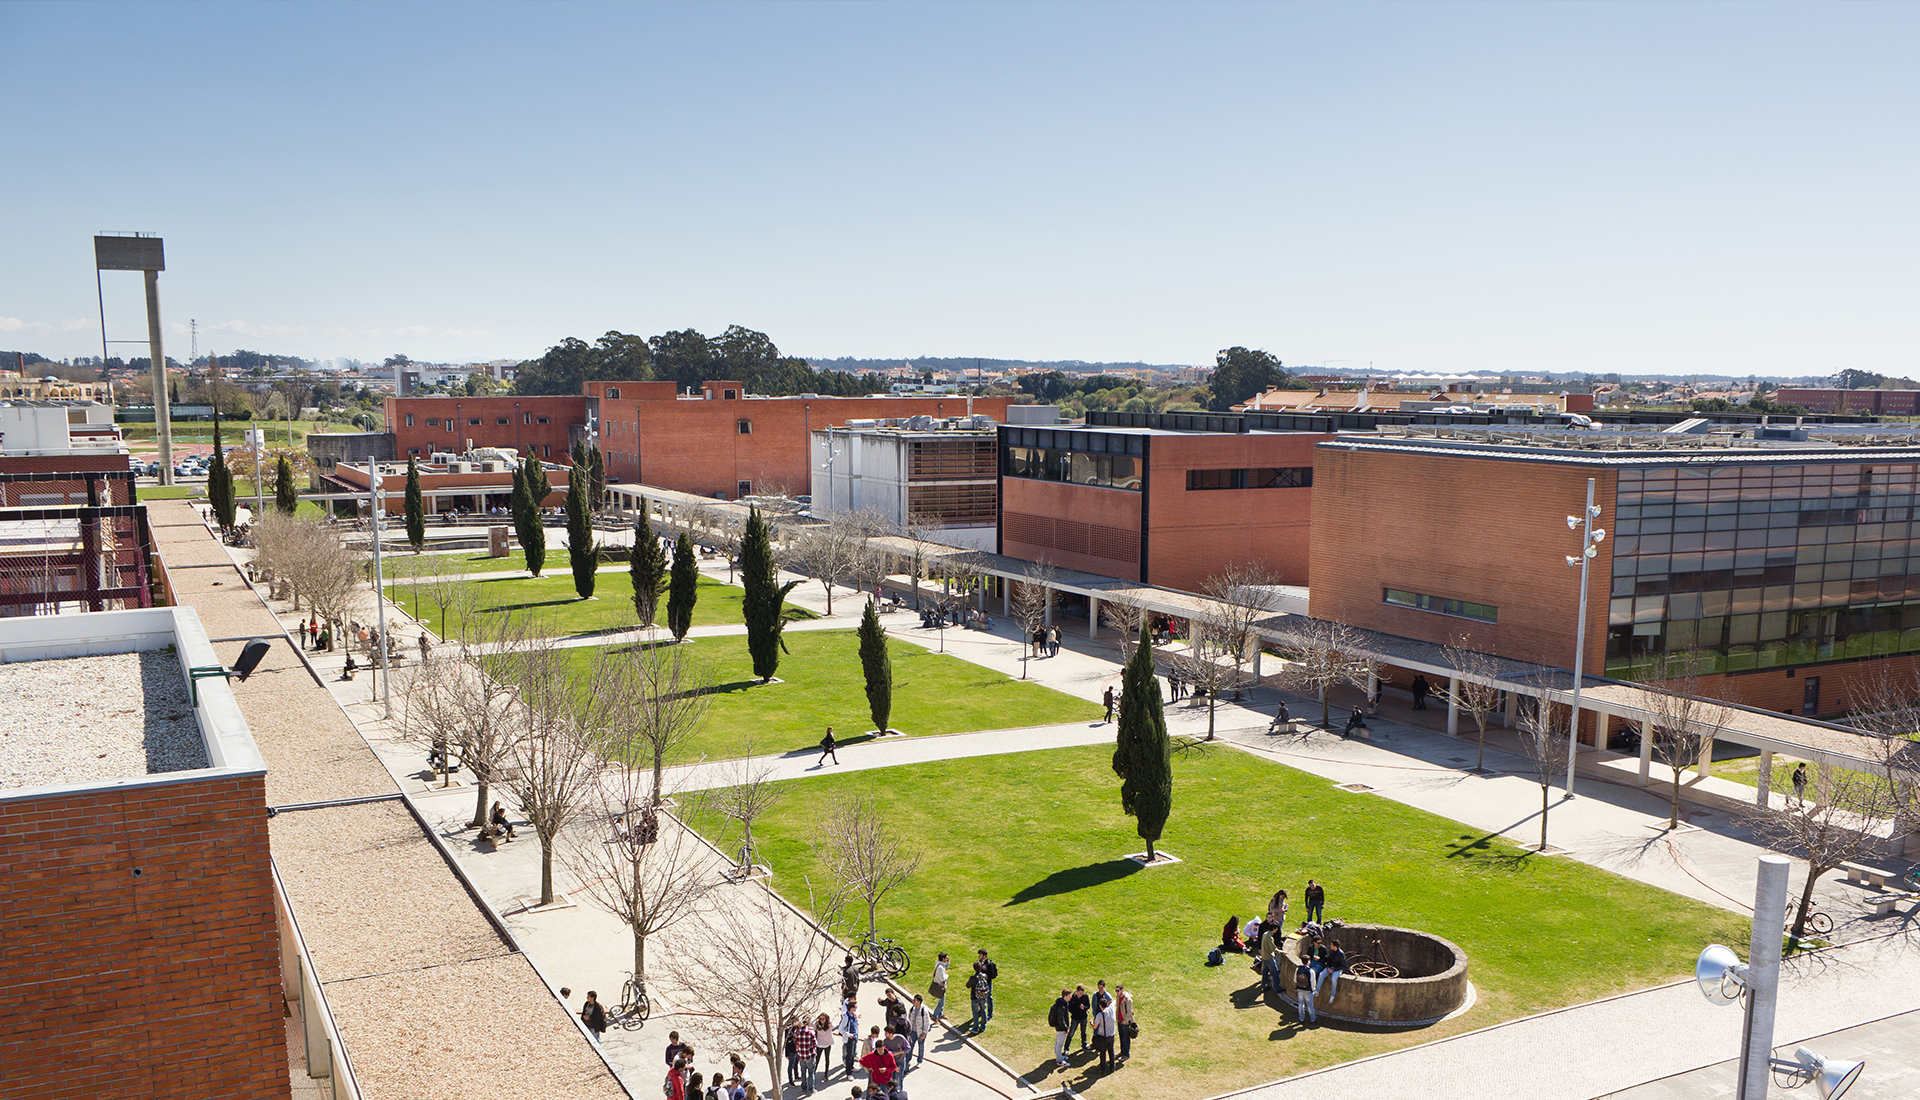
\includegraphics[width=4cm, height=5cm, angle=30]{Campus}
\end{lstlisting}

A imagem utilizada em cima irá agora aparecer distorcida.

\centering
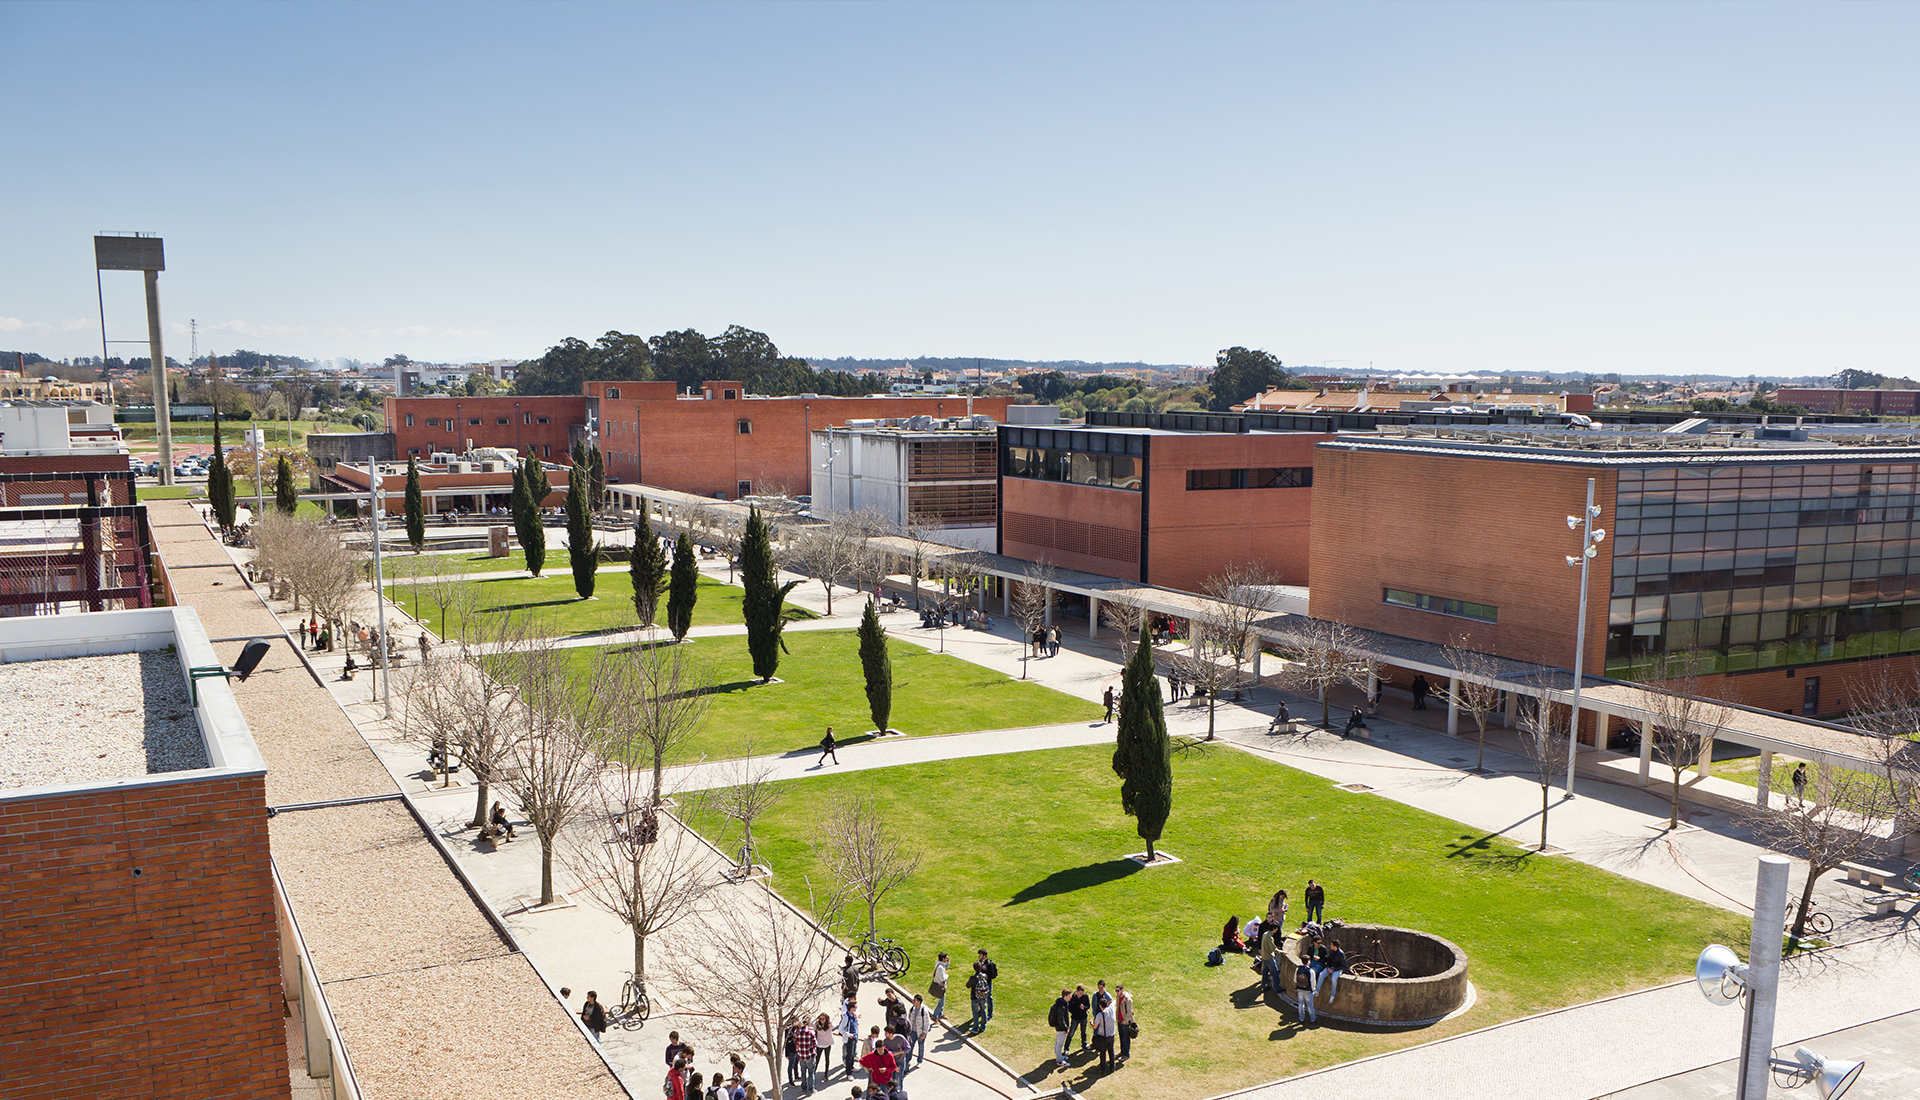
\includegraphics[width=4cm, height=5cm, angle=30]{Campus}

\RaggedRight
\vspace{5mm}
Mais informação sobre a inserção de imagens e sua formatação em {\LaTeX} encontra-se disponível nos fóruns de ajuda do WebSite \textit{\textbf{ShareLaTeX}}.\\
\url{https://www.sharelatex.com/learn/Inserting_Images}
\clearpage




\chapter{Conclusões}
\label{chap.conclusao}
Depois de uma extensa exploração das funcionalidades do {\LaTeX} é possível concluir que boas práticas ao redigir um documento de texto, tornam a tarefa mais fácil, tanto para o redator, como para o leitor. Apesar de conter muita informação, este documento de ajuda para {\LaTeX} apenas cobre a superfície das funcionalidades deste. No entanto, da \textit{"pouca"} informação que está contida neste documento, é possível reconhecer que {\LaTeX} oferece ao utilizador um maior controlo sobre o documento a ser redigido, comparativamente a editores de texto mais comuns, e, quantas mais funcionalidades forem aprendidas e usadas pelo redator, mais essa diferença será evidente, especialmente ao nível da apresentação e formatação do documento.

\chapter*{Contribuições dos autores}
As contribuições dos autores para este documento foram:

\begin{description}
	\item[\acrshort{RR}] - Introdução, Capítulos 2 e 4, Contribuições dos autores, acrónimos e glossário, bibliografia, pesquisa de informação;
	\item[\acrshort{JS}] - Resumo, Capítulos 3 e 5, conclusão, pesquisa de informação;
\end{description}

Como tal, e também com base nas estatísticas das revisões do code.ua, pode-se afirmar que a percentagem de contribuição de cada um foi:

\begin{description}
	\item[\acrshort{RR}] - 50\%
	\item[\acrshort{JS}] - 50\%
\end{description}

%%%%%%%%%%%%%%%%%%%%%%%%%%%%%%%%%

\printglossary[type=\acronymtype,title={Acrónimos e Abreviaturas}] % Apresenta o glossario de acronimos

\printglossary[title={Glossário}]

\printbibliography

\end{document}
